\RequirePackage{luatex85}
\PassOptionsToPackage{shorthands=off}{babel}
\makeatletter
\disable@package@load{fontenc}
\makeatother
\let\oldlooseness=\looseness
\documentclass{csbulletin}
\selectlanguage{czech}
\usepackage{titlesec}
\titlelabel{\thetitle\enspace}
\usepackage{luavlna}
\usepackage[strict]{lua-widow-control}
\usepackage{csquotes}
\usepackage[
  backend=biber,
  style=iso-numeric,
  sortlocale=cs,
  autolang=other,
  bibencoding=UTF8,
  mincitenames=2,
  maxcitenames=2,
  doi=false,
  isbn=false,
  shortnumeration=true,
]{biblatex}
\renewcommand\multicitedelim{\addsemicolon\space}
\addbibresource{main.bib}
\usepackage[
  implicit=false,
  hidelinks,
]{hyperref}
\usepackage{hologo}

\newcommand\acro[1]{\textsc{\MakeLowercase{#1}}}
\newcommand\pkg{\textsf}
\makeatletter
\newcommand\blfootnote[1]{%
  \begingroup
  \renewcommand\@makefntext[1]{\leftskip=0pt\relax#1}%
  \footnotetext{#1}%
  \endgroup
}
\def\strankasclankem#1#2{%
  \begingroup
  \def\csbul@start@page##1{%
    ##1%
    \endinput
    \ignorespaces
  }%
  \makeatletter
  \IfFileExists{../#1/#2.info}{\input ../#1/#2.info\relax}{\textbf{???}}%
  \endgroup
}
\makeatother

\begin{document}

\singlechars{czech}{AaIiVvOoUuSsZzKk}

\title{\CSTUG{} na konferenci TUG 2023}
\EnglishTitle{\CSTUG{} at the TUG 2023 Conference}
\author{Vít Starý Novotný}
\podpis{Vít Starý Novotný, witiko@mail.muni.cz}
\maketitle

\vspace*{-0.75cm}

\blfootnote{Tento článek byl původně zveřejněn jako zpráva na webu sdružení \CSTUG~\cite{starynovotny2023cstug}.}

\begin{figure}[b!]
\centering
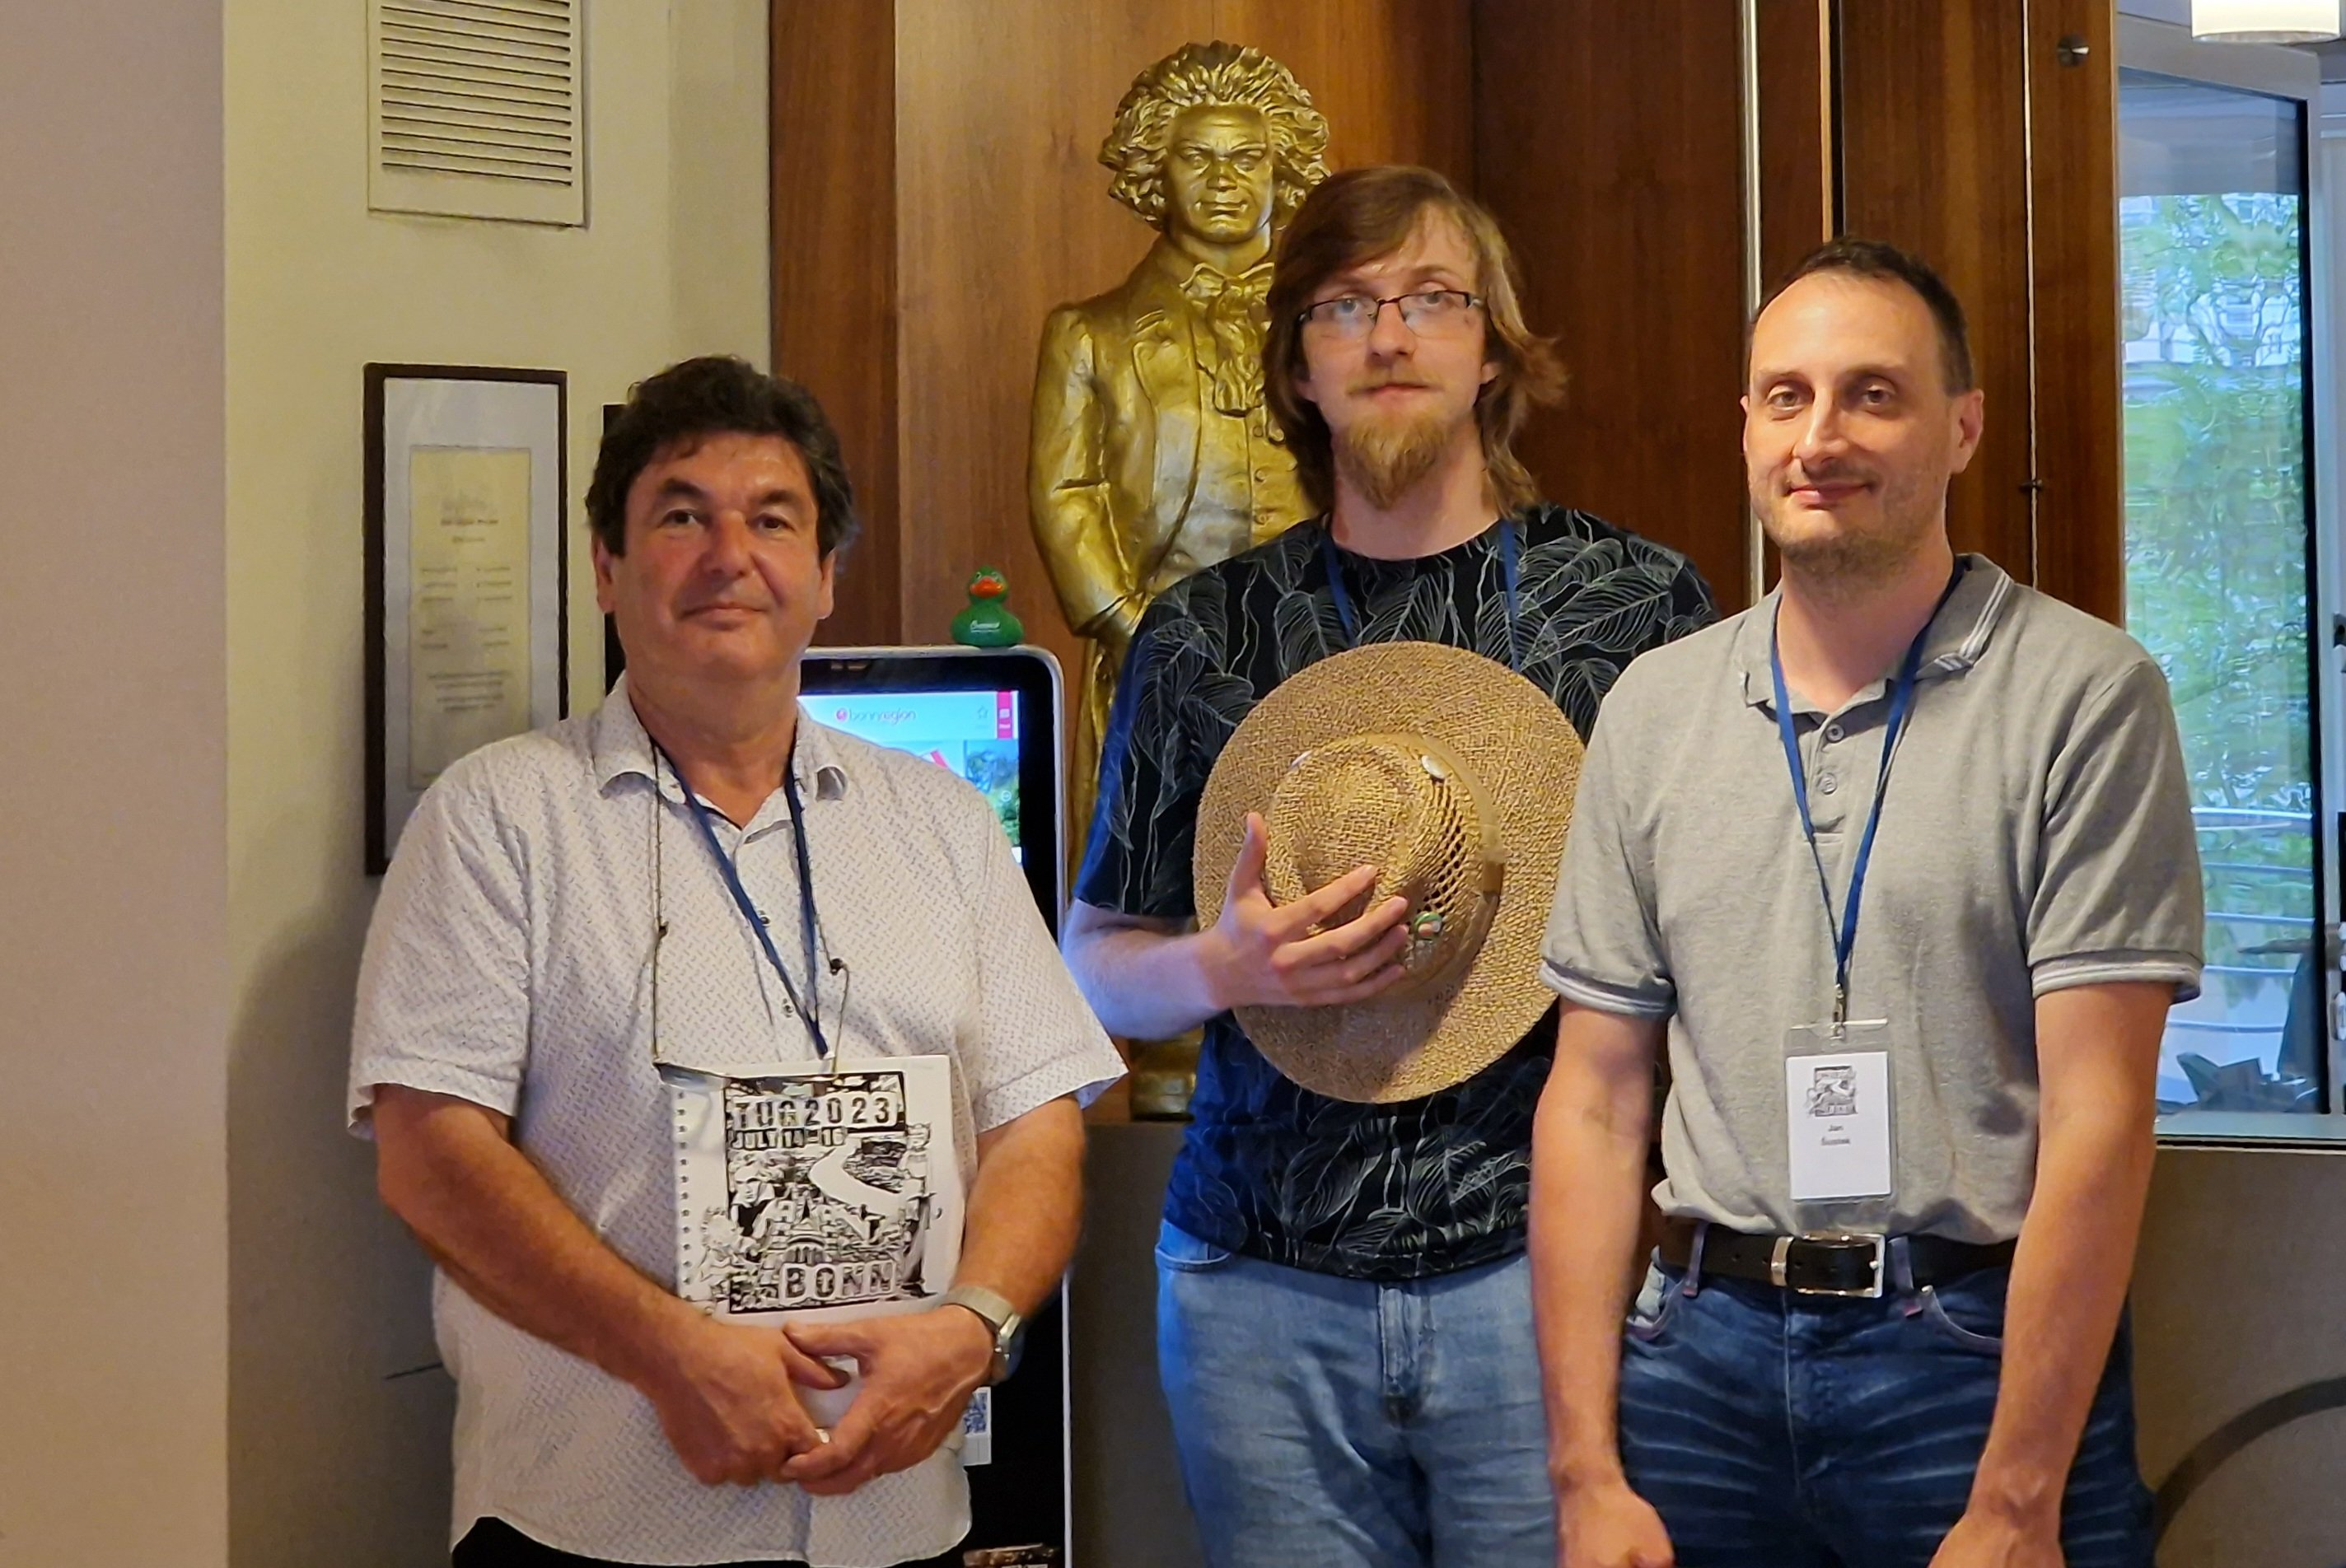
\includegraphics[width=0.7\linewidth]{figs/20230715_182848}
\caption{Petr Sojka (vlevo), Vítek Starý Novotný (uprostřed) a Honza Šustek (vpravo) na recepci konferenčního hotelu TUGu 2023}
\label{fig:cstug-attendees}
\end{figure}

Od pátku 14.\,července do neděle 16.\,července se v německém Bonnu konala konference TUG 2023. Konference se s podporou sdružení \CSTUG{} zúčastnili tři jeho členové: předseda Petr Sojka, technický redaktor Zpravodaje Vítek Starý Novotný a šéfredaktor Zpravodaje Honza Šustek, vizte Obrázek~\ref{fig:cstug-attendees}.

V pátek ráno představil Honza Šustek svůj makrobalík pro literární programování pomocí maker OPmac v přednášce nazvané \emph{On generating documented source code by blocks in \TeX{}}~\cite{sustek2023on}. Během přednášky položil Honza obecenstvu několik otázek. Tři šťastní řešitelé si po přednášce mohli připravit bylinný čaj pro Ostravu. Článek o Honzově přednášce si můžete přečíst na straně \strankasclankem{Sustek-literate}{main}.

Téhož dne večer představili Petr Sojka, Ondřej Sojka a Jakub Máca novinky z projektu univerzálních vzorů dělení slov v přednášce nazvané \emph{Universal syllabic pattern generation}~\cite{sojka2023roadmapa, sojka2023roadmapb}. V první části představil Ondřej Sojka technické a jazykové aspekty automatického dělení slov. V druhé části popsal Petr Sojka výsledky přípravy univerzálních vzorů pro devět jazyků a technická omezení programu Patgen, která zamezují generování vzorů pro více jazyků. V závěrečné části představil Jakub Máca datovou strukturu Judy, které se věnoval ve své bakalářské práci~\cite{maca2023judy} a kterou lze použít místo trií pro urychlení generování vzorů.

V sobotu ráno představil Vítek Starý Novotný třetí verzi makrobalíku pro přípravu dokumentů ve značkovacím jazyce Markdown v přednášce nazvané \emph{Markdown 3: What's new, what's next?}~\cite{novotny2023markdowna, novotny2023markdownb}. V první části přednášky Vítek představil nové funkce, které do balíku přibyly během posledních dvou let. V druhé části přednášky se Vítek zaměřil na nedostatky, které je třeba vyřešit před vydáním stabilní verze 3.0.0, a na nové funkce, které jsou plánované po vydání verze 3.0.0. Článek o Vítkově přednášce si můžete přečíst na straně \strankasclankem{StaryNovotny-markdown}{main}.

V neděli dopoledne proběhlo na závěr konference slosování výherců třetího vydání dvousvazkového díla The \LaTeX{} Companion~\cite{mittelbach2023latex}. Šťastným výhercem se stal i Honza Šustek, který si nechal knihy podepsat od přítomných členů \LaTeX ového týmu a pod tíhou distopie 1984 stran \LaTeX u odspěchal na vlak.

\vspace*{-0.25cm}
\section*{\refname}
\vspace*{-0.25cm}
\begingroup
\sloppy
\printbibliography[heading=none]
\endgroup

\vspace*{-0.25cm}
\begin{summary}
\vspace*{-0.25cm}
\oldlooseness=-1
This article reports on the participation of \CSTUG{} members at TUG 2023 in Bonn.
\end{summary}
\end{document}
